\documentclass[14pt,a4paper]{extarticle}
\usepackage[utf8]{inputenc}
\usepackage[russian]{babel}

% геометрия страницы
\usepackage{geometry}
\geometry{top=2cm, right=2.5cm, bottom=2cm, left=3cm}

% математика, графики, объединение ячеек, листинг
\usepackage{amsmath}
\usepackage{graphicx}
\graphicspath{{images/}}
\usepackage{multirow}
\usepackage{verbatim}

% межстрочные отступы и шрифты
\usepackage{setspace}
\usepackage{pscyr}

% подписи рисунков и таблиц по ГОСТу
\usepackage{caption}
\DeclareCaptionLabelFormat{figure}{Рисунок #2}
\DeclareCaptionLabelFormat{table}{Таблица #2}
\DeclareCaptionLabelSeparator{sep}{~---~}
\captionsetup{labelsep=sep,justification=centering,font=small}
\captionsetup[figure]{labelformat=figure}
\captionsetup[table]{labelformat=table}

% ссылки в pdf-файле
\usepackage{color}
\usepackage[colorlinks,linkcolor=black,urlcolor=black]{hyperref}
\renewcommand{\UrlFont}{\rm\small}

% центрированный столбец заданной ширины (в процентах от ширины страницы)
\usepackage{array}
\newcolumntype{C}[1]{>{\centering\arraybackslash}m{#1\textwidth}}
\renewcommand{\arraystretch}{1.2}

\begin{document}
  \begin{titlepage}
    \singlespacing
    \begin{center}
      Министерство образования и науки Российской Федерации \\
      Федеральное государственное бюджетное образовательное \\
      учреждение высшего профессионального образования \\
      <<Волгоградский государственный технический университет>> \\
      Факультет электроники и вычислительной техники \\
      Кафедра физики
    \end{center}

    \vspace{9em}

    \begin{center}
      \large Семестровая работа по дисциплине \\
      <<Радиоэлектроника>>
    \end{center}

    \vspace{5em}

    \begin{flushright}
      \begin{minipage}{.40\textwidth}
        Выполнили \\
        студенты группы Ф-469 \\
        Слоква В. И., \\
        Чечеткин И. А. \\

        \vspace{1em}

        Проверил профессор, \\
        доктор физ.-мат. наук \\
        Смоляр В. А.
      \end{minipage}
    \end{flushright}

    \vspace{\fill}

    \begin{center}
      Волгоград, \the\year
    \end{center}
  \end{titlepage}

  \setcounter{page}{2}
  \tableofcontents
  \newpage

  \section*{Параметры полупроводника}
  \addcontentsline{toc}{section}{Параметры полупроводника}

  \begin{table}[h!]
    \center
    \caption{Параметры полупроводника}
    \begin{tabular}{|l|C{.2}|} \hline
      \multicolumn{2}{|c|}{\bf Кремний (Si)} \\ \hline
      Эффективная масса электронов & \( 1,\!08 \cdot m_e \) \\
      Эффективная масса дырок & \( 0,\!56 \cdot m_e \) \\
      Энергия дна зоны проводимости,~эВ & \( 4,\!02 \) \\
      Энергия вершины валентной зоны,~эВ & \( 5,\!23 \) \\
      Ширина запрещенной зоны,~эВ & \( 1,\!21 \) \\ \hline
    \end{tabular}
  \end{table}

  \newpage

  \section{Концентрация электронов и дырок в собственном полупроводнике}

  Концентрация электронов в зоне проводимости равна:
  \begin{equation}
    n = 2\cdot\int\limits_{E_C}^\infty N(E) f(E, T) dE.
    \label{G1.9}
  \end{equation}

  Если уровень Ферми \( F \) лежит в запрещенной зоне энергий и удален от края
  зоны \( E_C \) хотя бы на \( 2kT \), то в распределении Ферми-Дирака
  \eqref{G1.7}
  \begin{equation}
    f(E, T) = \frac{1}{1 + e^{\dfrac{E - F}{kT}}}
    \label{G1.7}
  \end{equation}
  единицей в знаменателе можно пренебречь и оно переходит в распределение
  Максвелла-Больцмана классической статистики (для кремния показаны на
  рис.~\ref{picF}). Это случай невырожденного полупроводника:
  \begin{equation}
    f(E, T) = e^{-\dfrac{E - F}{kT}}.
    \label{G1.8}
  \end{equation}

  \begin{figure}[h!]
    \center
    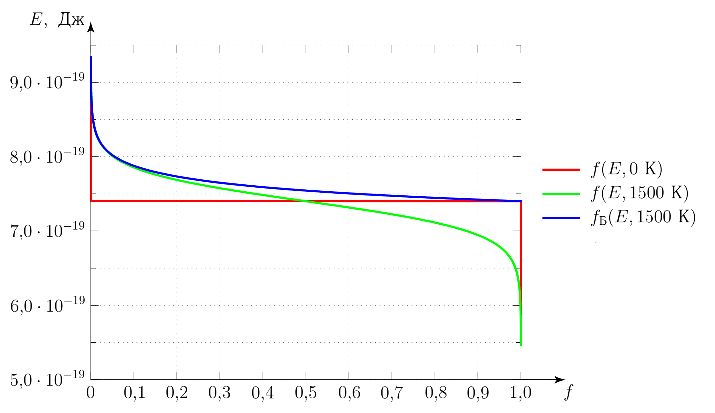
\includegraphics[width=.75\textwidth]{f(1500K)}\\
    \caption{Функции Ферми-Дирака \( f \) и Больцмана \( f_\emph{Б} \) для
      температуры 1500 К}
    \label{picF}
  \end{figure}

  Плотность состояний в зоне проводимости \( N(E) \) выражается формулой
  \begin{equation}
    N(E) = \frac{4\pi m_n^{3/2}\cdot\sqrt{2(E - E_C)}}{h^3},
    \label{G1.6}
  \end{equation}
  где \( m_n^{3/2} \)~-- эффективная масса электрона, \( E_C \)~-- энергия,
  соответствующая дну зоны проводимости.

  Если вместо \( (E - E_C) \) подставить \( (E_V - E) \), а вместо \( m_n \)~--
  эффективную массу дырки \( m_p \), то получим формулу плотности состояний в
  валентной зоне.

  Для кремния \( N(E) \) выглядит так, как показано на рисунке~\ref{picNE}.
  \begin{figure}[ht]
    \center
    \includegraphics[width=.75\textwidth]{N(E)}
    \caption{Функция распределения плотности состояний в зоне проводимости
      \( N(E) \)}
    \label{picNE}
  \end{figure}

  \begin{figure}[b!]
    \center
    \includegraphics[width=.75\textwidth]{ni}
    \caption{Зависимость \( n_i(T) \), \( N_C(T) \), \( N_V(T) \)}
    \label{picNi}
  \end{figure}

  Подставив \eqref{G1.8} и \eqref{G1.6} в \eqref{G1.9}, получим:
  \begin{equation}
    n = N_C\cdot e^{-\dfrac{E_C - F}{kT}},
    \label{G1.10}
  \end{equation}
  где \( N_C \) -- эффективная плотность состояний в зоне проводимости:
  \[
    N_C = 2\cdot\left (\frac{2\pi m_n kT}{h^2} \right)^{3/2}.
  \]

  Концентрация дырок в валентной зоне:
  \begin{equation}
    p = N_V\cdot e^{-\dfrac{F - E_V}{kT}},
    \label{G1.13}
  \end{equation}
  где \( N_V \) -- эффективная плотность состояний в валентной зоне:
  \[
    N_V = 2\cdot\left (\frac{2\pi m_p kT}{h^2} \right)^{3/2}.
  \]

  Для расчета \( n \) и \( p \) по уравнениям \eqref{G1.10} и \eqref{G1.13}
  необходимо знать положение уровня Ферми \( F \). Однако произведение
  концентраций электронов и дырок для невырожденного полупроводника не зависит
  от уровня Ферми, хотя зависит от температуры:
  \begin{equation}
    n\cdot p = (n_i)^2 = N_C\cdot N_V\cdot e^{-\dfrac{E_g}{kT}}.
    \label{G1.14}
  \end{equation}

  Концентрацию собственных носителей заряда в зоне проводимости и в валентной
  зоне рассчитаем из формулы \eqref{G1.14}. Для кремния зависимость
  \( n_i(T) \), \( N_C(T) \), \( N_V(T) \) отображена на рисунке~\ref{picNi}.

  \newpage

  \section[Код программы]{Код программы на C (с использованием gnuplot)}
  {\small
  \verbatiminput{code.c}
  }

  \newpage

  \begin{thebibliography}{9}
    \addcontentsline{toc}{section}{Список литературы}
    \bibitem{1} Гуртов,~В.~А. Твердотельная электроника: Учеб. пособие~/
      В.~А.~Гуртов.~-- М., 2005.~-- 492~с.
    \bibitem{2} NSM Archive~-- Physical Properties of Semiconductors \\
      \url{http://www.matprop.ru/semicond}
  \end{thebibliography}

\end{document}